\section{ETVOIP}
In the ETVOIP tab of a virtual machine that, has the solution installed, we are enabled to manage a VOIP solution ETVOIP.
Currently ETVOIP is the interaction with the PBX component and may interact with other future developments.
The available modules for this agent are:

\begin{itemize}
    \item Extensions
    \item Trunks
    \item Outbound routes
    \item Inbound routes
\end{itemize}


\begin{quote}
	{\large \bf Note} \\*[-.8pc]
	\underline{\hspace{6in}} \\
    At the end of all operations/changes you should use the \emph{Apply changes} button available in any of the modules, in order to reflect these changes in the current configuration of the VOIP system.
\end{quote}


\begin{figure}[H]
        \begin{center}
        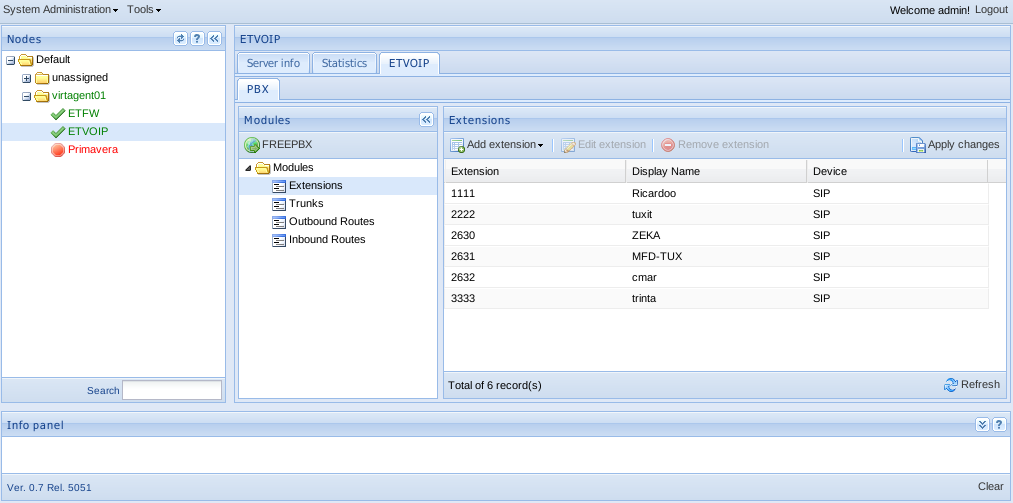
\includegraphics[scale=0.45]{screenshots/etvoip_pbx.png}
        \caption{Main ETVOIP panel management}
        \label{fig:etvoip_pbx}
        \end{center}
\end{figure}

In addition to these modules there is also the option to open a window FREEPBX alone, having access to advanced settings (Menu FREEPBX).

\subsection{Extensions}

In extensions pane it's possible to add, edit an remove extensions.

\begin{quote}
	{\large \bf Note} \\*[-.8pc]
	\underline{\hspace{6in}} \\
    You can only create/edit SIP extensions \footnote{SIP is a standard protocol designed for VoIP devices} and/or IAX\footnote {IAX it's the protocol "Inter Asterisk" used to interconnect asterisk servers.}.
\end{quote}

\begin{figure}[H]
        \begin{center}
        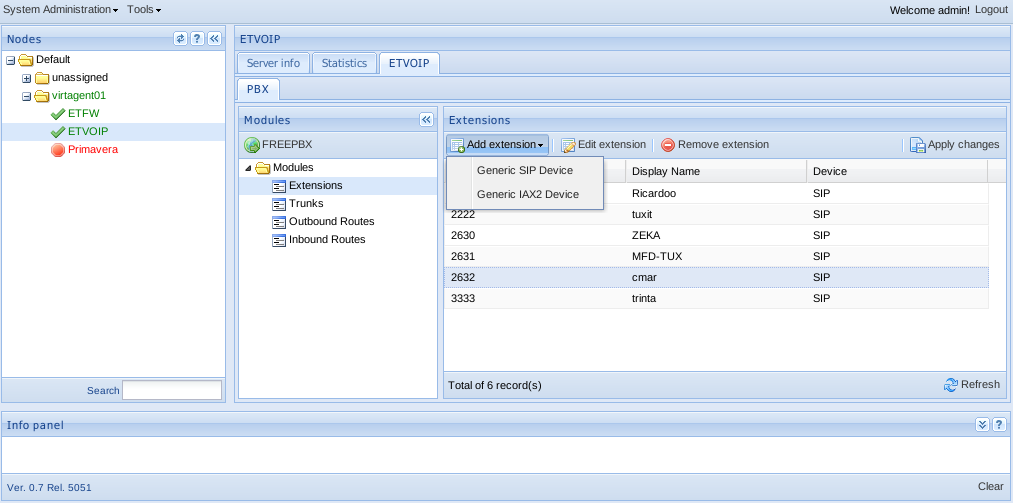
\includegraphics[scale=0.45]{screenshots/etvoip_pbx_extensions.png}
        \caption{Extension management panel}
        \label{fig:etvoip_pbx_extensions}
        \end{center}
\end{figure}


\subsubsection{Add extension}
\label{sec:etvoip_pbx_extensions_add}
When creating an extension is possible to choose between the basic/advanced settings view.

\begin{figure}[H]
        \begin{center}
        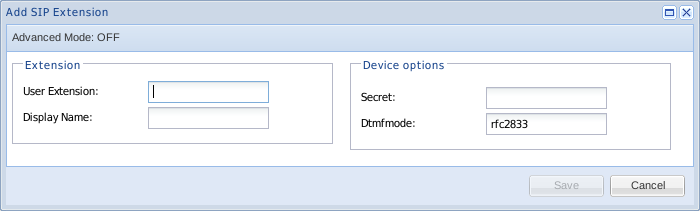
\includegraphics[scale=0.6]{screenshots/etvoip_pbx_extensions_sip.png}
        \caption{Add extension window (SIP)}
        \label{fig:etvoip_pbx_extensions_sip}
        \end{center}
\end{figure}


\begin{description}
	\item[Advanced mode: OFF -] This mode is available only the basic fields to create an extension.
        \begin{description}
            \item[Extension -] Extension parameters.
                \begin{itemize}
                    \item User extension - User extension number. Must be unique.
                    \item Display name - User name shown on his calls. Introduce a name, not a number.
                \end{itemize}

            \item[Device options -] Options for the type of device chosen.
                \begin{itemize}
                    \item Secret - Password that devices must use to authenticate on the asterisk server.
                    \item Dtmfmode - Multi Dual-Tone frequency.
                        \begin{itemize}
                            \item inband - The sending device generates DTMF tones.
                            \item outband - The ring tones are removed from the audio data and sent from a different channel.
                            \item rfc2833 - Specify a format for sending RTP packets, in order to reduce the transmitted data. Used by default.
                        \end{itemize}
                \end{itemize}
        \end{description}
	\item[Advanced mode: ON -] In this mode beyond the parameters mentioned above you can configure the following:
        \begin{description}
            \item[Extension -] Configuration parameters for extension configuration.
                \begin{itemize}
                    \item Alternative CID number - CID number to be used for internal calls, if different from the extension number. Used to masquerade as a different user. A common example is when a support team need to have your internal caller ID to show the overall number of support. Has no effect on incoming calls.
                    \item Alternative SIP - If you want to support direct sip calls to internal users or through anonymous sip calls, can provide a friendly name that can be used instead of the user's extension.
                \end{itemize}

            \item[Extension options -] Advanced extension options.
                \begin{itemize}
                    \item Outbound CID - Replaces the caller ID if passes a trunk. Overrides the outbound CID of the trunk.
                    \item Ring time - Number of seconds ringing before sending the caller to voicemail. If you do not have voicemail set this parameter is ignored.
                    \item Call waiting - Sets the initial state of call waiting for this extension 
                    \item Call screening - Requires the caller to say his name, which is then heard by the user, allowing him to accept or reject the call. Memory Screening (\emph{Screen Caller:Memory}) checks only once the source of the caller ID. Screening without memory (\emph{Screen Caller: No Memory}) always requires that the external user say his name. Either way will announce whenever the user from the last entry saved with this caller ID.
                    \item Pinless dialing - Enabled allows you to make outgoing calls from this extension without dialing PIN.
                    \item Emergency CID - This caller ID is used whenever you select an exit route marked out as an emergency. The Emergency CID overrides all other settings the caller ID.
                \end{itemize}

            \item[Assigned DID/CID -] Definition of the incoming route for this extension.
                \begin{itemize}
                    \item DID description - Incoming route description.
                    \item Add inbound DID - Sets the incoming number associated with this extension (Direct Inward Dialing).
                    \item Add inbound CID - Allows you to specify a best route DID + CID. DID should be specified in the above parameter.
                \end{itemize}

            \item[Voicemail \& Directory -] Voicemail parameters.
                \begin{itemize}
                    \item Status - Enable/disable this voicemail extension.
                    \item Voicemail Password - Password to access the voicemail system. The password can only contain numbers. A user can change the password after accessing the voicemail system (*98) in his voip phone.
                    \item Email Address - Email address of destination where voicemail notifications are sent.
                    \item Pager Email Address - Email address (pager/mobile) phone for sending  voicemail notifications.
                    \item Email Attachment - Allows you to attach voicemails to email.
                    \item Play CID - Read the phone number of origin before playing the incoming message.
                    \item Play Envelope - Read the date/time of the message.
                    \item Delete Voicemail - If enabled the message will be deleted from voicemail (after AIDS mailed). Allows a user to get his voicemail via email, without having to retrieve voicemail via the web interface or phone. CAUTION: It needs to have voicemail attached to the email, otherwise the messages will be lost.
                    \item IMAP Username - IMAP username, if in use.
                    \item IMAP Password - IMAP password.
                    \item VM Options - Extra voicemail options separated by | (such as review = yes | maxmessage = 60).
                    \item VM Context - Context used by the voicemail system. Use 'default' if you do not know the implications.
                \end{itemize}

            \item[Dictation services -] Parameters for diction service. If enabled, allows the user to dial *34 from his phone and record the conversation. The speech will be record in the defined format and sent to the specified e-mail.
                \begin{itemize}
                    \item Dictation Device
                    \item Dictation Format
                    \item Email Address
                \end{itemize}

            \item[Language -] Parameters of the extension language.
                \begin{itemize}
                    \item Language Code - If installed, it will ask if the user want to use the selected language.
                \end{itemize}

            \item[Recording options -] Extension recording parameters.
                \begin{itemize}
                    \item Record Incoming - Record all incoming calls from this extension.
                    \item Record Outgoing - Record all outgoing calls from this extension.
                \end{itemize}
            
        \end{description}
\end{description}

\subsubsection{Edit an extension}

To edit an extension is necessary to select the desired extension and click on button \emph{Edit extension}. Then you will see a window (see Figure \ref{fig:etvoip_pbx_extensions_sip}) filled with the extension's settings.
The parameters are identical to those provided in section \ref{sec:etvoip_pbx_extensions_add}.

\subsubsection{Remove an extension}
Select the extension to be removed and then click on \emph{Remove extension} button.
A window will appear confirming the removal (Figure \ref{fig:etvoip_pbx_extensions_remove}). After removing the extension and if you do not want to perform any other operation, you must apply the changes made in button \emph{Apply changes}.

\begin{figure}[H]
        \begin{center}
        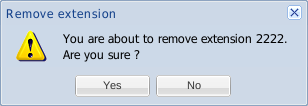
\includegraphics[scale=0.6]{screenshots/etvoip_pbx_extensions_remove.png}
        \caption{Remove an extension}
        \label{fig:etvoip_pbx_extensions_remove}
        \end{center}
\end{figure}

\subsection{Trunks}

In the section \emph{Trunks} you do add/edit and remove operations.

\begin{quote}
	{\large \bf Note} \\*[-.8pc]
	\underline{\hspace{6in}} \\
    It's only possible to create/edit SIP/IAX trunks.
\end{quote}

\begin{figure}[H]
        \begin{center}
        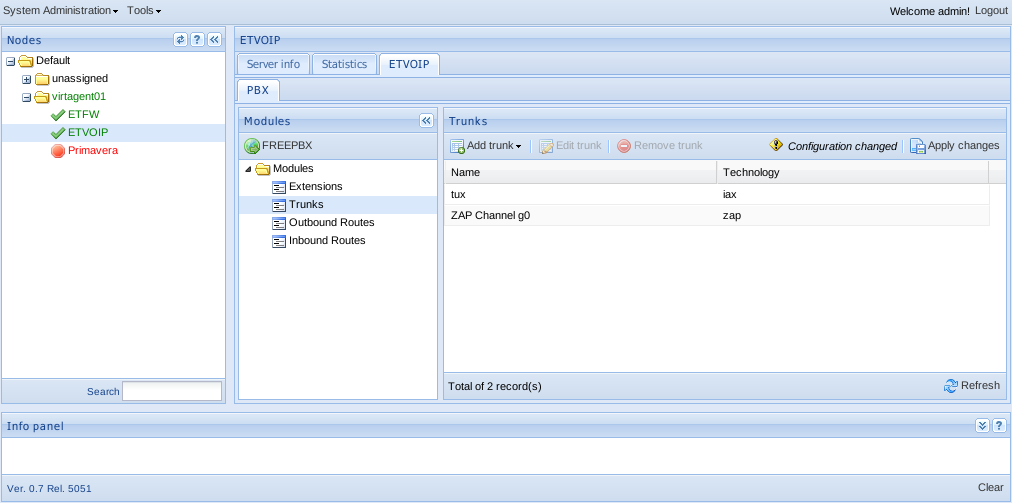
\includegraphics[scale=0.45]{screenshots/etvoip_pbx_trunks.png}
        \caption{Trunk management panel}
        \label{fig:etvoip_pbx_trunks}
        \end{center}
\end{figure}

\subsubsection{Add Trunk}
\label{sec:etvoip_pbx_trunks_add}
When creating a trunk you can choose between the basic or advanced view by pressing the top left button.

\begin{figure}[H]
        \begin{center}
        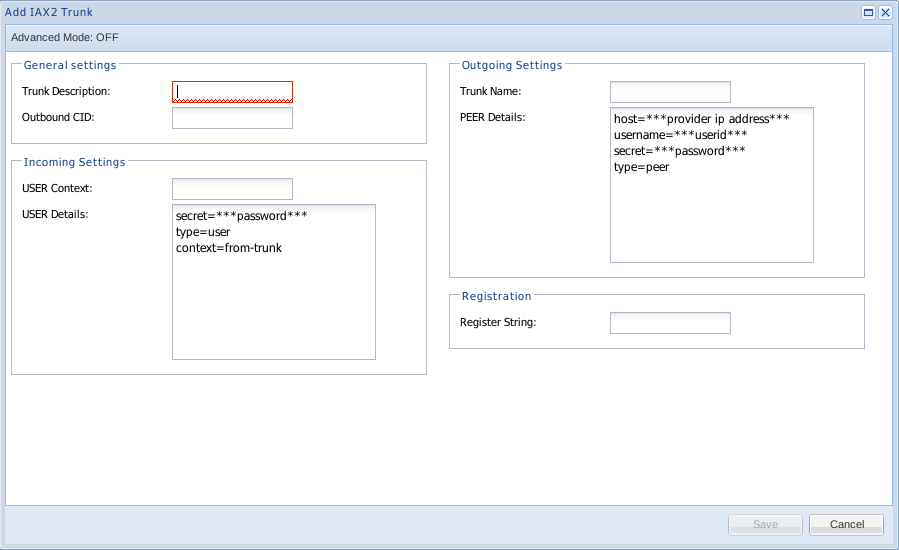
\includegraphics[scale=0.45]{screenshots/etvoip_pbx_trunks_iax.png}
        \caption{IAX2 trunk creation window}
        \label{fig:etvoip_pbx_trunks_iax}
        \end{center}
\end{figure}


\begin{description}
	\item[Advanced mode: OFF -] This mode only show the basic fields needed in order to create a trunk.
        \begin{description}
            \item[General settings -] Trunk parameters.
                \begin{itemize}
                    \item Trunk description - Name that better describes the trunk.
                    \item Outbound CID - Call identifier used in calls made through this trunk.
                \end{itemize}

            \item[Incoming setting -] Input configurations.
                \begin{itemize}
                    \item USER Context - This is usually the account name or number that the provider is waiting. This USER Context is used to define the details of the user outlined below.
                    \item USER Details - User connection parameters to the VOIP system.
                \end{itemize}
            \item[Outgoing setting -] Output configurations.
                \begin{itemize}
                    \item Trunk name - Unique name of the trunk.
                    \item PEER details - Connection parameters between the PEER and the VOIP system.
                \end{itemize}
            \item[Registration -] VOIP registration parameters.
                \begin{itemize}
                    \item Register string - Many VoIP providers require the system to REGISTER. Enter the online registration here (example: username:password@switch.voipprovider.com). Many providers require a DID number (ex: username:password@switch.voipprovider.com/didnumber) to work the match DID
                \end{itemize}
        \end{description}
	\item[Advanced mode: ON -] This mode shows the available advanced parameters.
        \begin{description}
            \item[General settings -] Advanced trunk parameters.
                \begin{itemize}
                    \item CID Options - Determines what CIDs are allowed on this trunk. IMPORTANT: CIDs emergency defined in an extension will always be used if the trunk is part of an emergency route regardless of the settings.
                        \begin{itemize}
                            \item Allow Any CID - All CIDs including those from external forwarded calls will be transmitted.
                            \item Block Foreign CIDs - Blocks forwarded CIDs. The defined CIDs will be transmitted.
                            \item Remove CNAM - This option will remove CNAM from each CID sent by this trunk.
                            \item Force Trunk CID - Always use the CID set to trunk unless it is part of an emergency route to an emergency CID set to an extension.
                        \end{itemize}                         
                    \item Maximum Channels - Controls the maximum number of output channels (simultaneous calls) that can be made in this trunk. Incoming calls are not considered. Leave blank to not specify a limit.
                    \item Disable Trunk - Disable the use of this trunk in all routes where it is used.
                    \item Monitor Trunk Failures - If enabled, enter the name of an AGI script to be used for logging, email, or perform any action in case of failure, if the failures are not caused by NOANSWER or CANCEL.
                \end{itemize}

            \item[Outgoing dial rules -] Advanced dial options.
                \begin{itemize}
                    \item Dial Rules - A dialing rule controls how calls will be marked in this trunk. It can be used to add or remove prefixes. If the numbers didn't match the standards setted here, they will be dialled with no change. A pattern without + or | (to add or remove a prefix) will not make changes but will create a match. Only the first match found will be performed:
                        \begin{itemize}
                            \item X - Pattern matching with digits from 0 to 9.
                            \item Z - Pattern matching with digits from 1 to 9.
                            \item N - Pattern matching with digits from 2 to 9.
                            \item [1237-9] - Pattern matching with number or letters between brackets (e.g. 1,2,3,7,8,9).
                            \item . - Wildcard, pattern matching with one or more chars (not allowed before | or +).
                            \item | - Removes a dial prefix (e.g., 613|NXXXXXX matches when someone dial "6135551234", but only "5551234" passes into the trunk).
                            \item + - Adds a dial prefix into the number (for example, 1613+NXXXXXX matches when someone dial "5551234", but only "16135551234" is passed into the trunk).
                        \end{itemize}
                        We can use, simultaneously, + and |, for example: 01+0|1ZXXXXXXXXX does match with "016065551234" and marks it as "0116065551234". Note that the order does not matter, ie, 0|01+1ZXXXXXXXXX does exactly the same thing.
                    \item Outbound Dial Prefix - The outbound prefix is used to put a prefix on all outgoing calls from this trunk. For example, if the trunk has behind another PBX, we can use 9 to access an outgoing line. Most users should leave the option blank.
                \end{itemize}
        \end{description}
\end{description}


\subsubsection{Edit Trunk}

To edit a trunk we need to select the trunk to remove and click on option \emph{Edit trunk}. Then we see a window (see Figure \ref{fig:etvoip_pbx_trunks_iax}) filled with the definitions of the trunk.
The parameters are identical to those provided in section \ref{sec:etvoip_pbx_trunks_add}.

\subsubsection{Remove trunk}

To remove a selected trunk click on \emph{Remove trunk} option.
A window will appear confirming removal of the trunk (Figure \ref{fig:etvoip_pbx_trunks_remove}). After removal of the trunk and if they do not want to perform any other operation, you must apply the changes made - \emph{Apply changes} option.

\begin{figure}[H]
        \begin{center}
        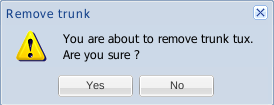
\includegraphics[scale=0.6]{screenshots/etvoip_pbx_trunks_remove.png}
        \caption{Remove trunk}
        \label{fig:etvoip_pbx_trunks_remove}
        \end{center}
\end{figure}


\subsection{Outbound routes}
The \emph{Outbound routes} configures the behavior of outgoing calls. The dialed number is analyzed, and a pattern matching is made in order to find the outbound route. After that the call is forwarded to the respective trunk.

You can add, edit and remove exit routes.

\begin{figure}[H]
        \begin{center}
        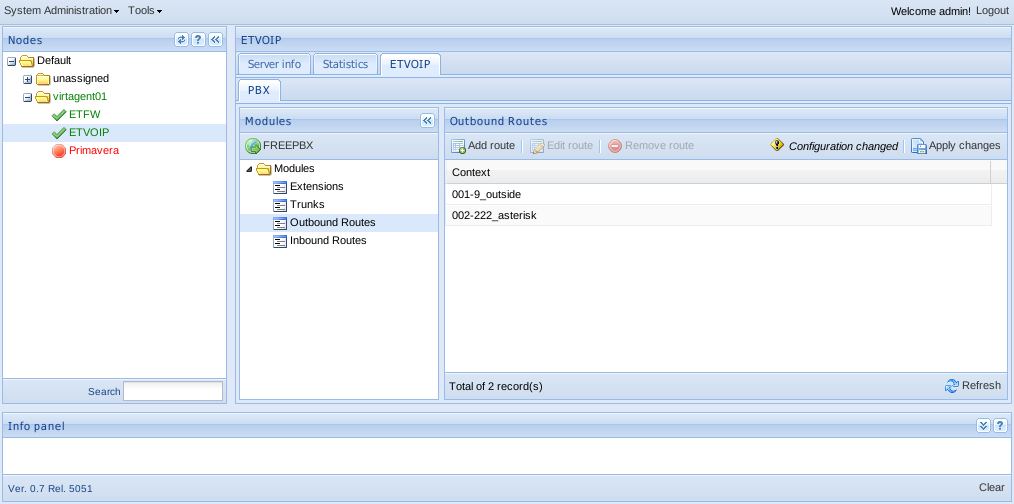
\includegraphics[scale=0.45]{screenshots/etvoip_pbx_outbound_routes.png}
        \caption{Outbound management panel}
        \label{fig:etvoip_pbx_outbound_routes}
        \end{center}
\end{figure}

\subsubsection{Add route}
\label{sec:etvoip_pbx_outbound_routes_add}

When you select the option \emph{Add route} a window will appear (see Figure \ref{fig:etvoip_pbx_outbound_routes_add}) where you can choose between the basic/advanced settings view setting mode. The following parameters are available:

\begin{description}
	\item[Advanced mode: OFF -] In this mode you can define the route basic settings.
        \begin{description}
            \item[General settings -] Route parameters.
                \begin{itemize}
                    \item Route Name - Route name (e.g., 'local').
                    \item Dial Patterns - Pattern that the dialing number must match to select this route:
                        \begin{itemize}
                            \item X - Pattern matching with digits from 0 to 9.
                            \item Z - Pattern matching with digits from 1 to 9.
                            \item N - Pattern matching with digits from 2 to 9.
                            \item [1237-9] - Pattern matching with number or letters between brackets (e.g. 1,2,3,7,8,9).
                            \item . - Wildcard, pattern matching with one or more chars (not allowed before | or +).
                            \item | - Removes a dial prefix (e.g., 613|NXXXXXX matches when someone dial "6135551234", but only "5551234" passes into the trunk).
                            \item / - Adds to the pattern. Does the match with a CID or pattern (e.g., NXXXXXX/104 matches only with the "104" extension).
                        \end{itemize}
                \end{itemize}

            \item[Trunks -] Sequence output trunks. The sequence of trunks control the order of trunks that will be used when the number matches the defined patterns.
        \end{description}
	\item[Advanced mode: ON -] This mode shows some additional configurations that can be made:
        \begin{description}
            \item[General settings -] Trunk parameters.
                \begin{itemize}
                    \item Route CID - If selected will re-write all specific CIDs except:
                        \begin{itemize}
                            \item Emergency CIDs (extension/device) if this route was marked as an emergency route.
                            \item Trunk CID if the trunk is marked to force the CID.
                            \item CIDs from forwarded calls (CF, Follow Me, Ring Groups, etc).
                            \item CIDs from extensions/users if enabled.
                        \end{itemize}                       
                    \item Route Password - The route can request the user to insert a password before allowing the call. Useful in cases of international call barring.
                       A numerical password, or the path to a file with the password to be used. Leave this field blank unless required for a password.
                    \item Emergency Dialing - Selecting this option will force the use of an emergency CID (if configured). This option allows that a given set of routes must been used to dial the emergency number (eg: 112).
                    \item Internal Company Route - By selecting this option the route will be treated as an intra-company connection, preserving the internal CID information and not using the output CID either the extension or trunk.
                    \item Music On Hold? - Defines the type of music when the call is on hold.
                \end{itemize}            
        \end{description}
\end{description}


\begin{figure}[H]
        \begin{center}
        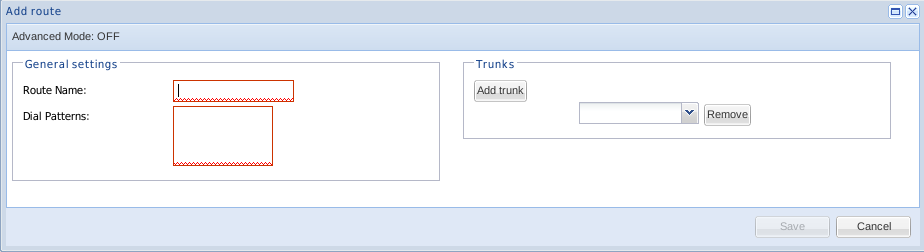
\includegraphics[scale=0.45]{screenshots/etvoip_pbx_outbound_routes_add.png}
        \caption{Add outbound route window}
        \label{fig:etvoip_pbx_outbound_routes_add}
        \end{center}
\end{figure}


\subsubsection{Edit route}
To edit an outbound route is necessary to select the desired route and click on \emph{Edit route}. Then you will see a window (see Figure \ref{fig:etvoip_pbx_outbound_routes_add}) filled with the definitions of the route.
The parameters are identical to those provided in section \ref{sec:etvoip_pbx_outbound_routes_add}.

\subsubsection{Remove route}
To remove a selected outbound route click on the \emph{Remove route} button.
A window will appear confirming the removal of the route (Figure \ref{fig:etvoip_pbx_outbound_routes_remove}). After the removal and if you do not want to perform any other operation, you must apply the changes made pressing the \emph{Apply changes} button.

\begin{figure}[H]
        \begin{center}
        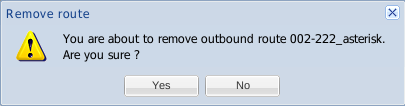
\includegraphics[scale=0.6]{screenshots/etvoip_pbx_outbound_routes_remove.png}
        \caption{Remove outbound route}
        \label{fig:etvoip_pbx_outbound_routes_remove}
        \end{center}
\end{figure}


\subsection{Incoming routes}
In \emph{Inbound Routes} we can configure the behavior of incoming calls of all trunks.
When receiving an incoming call, the VOIP server needs to know where to redirect it.
Can be redirected to a Ring Group, an extension or IVR, among other options.

Therefore, it is possible to perform operations to add, edit and remove routes of entry.
In the management panel you can view the description and the numbers DID/CID associated with each route.

\begin{figure}[H]
        \begin{center}
        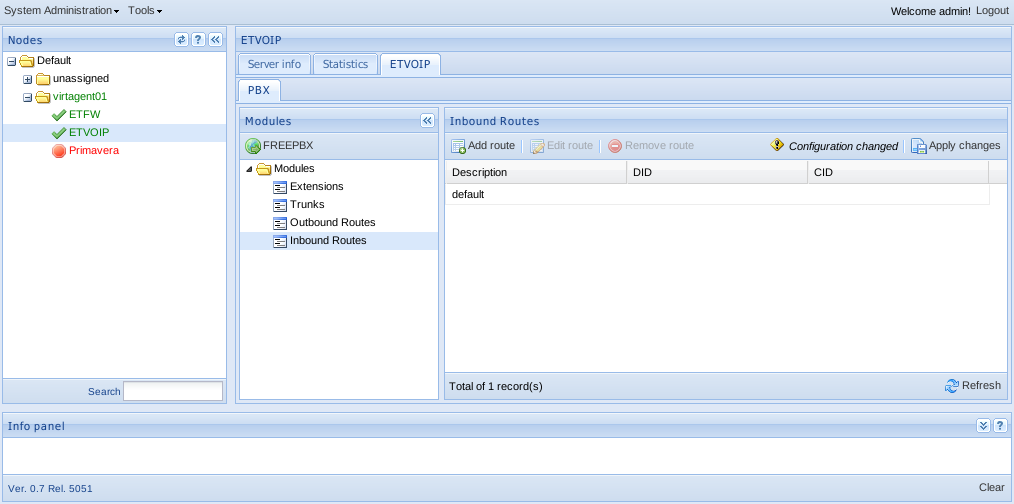
\includegraphics[scale=0.45]{screenshots/etvoip_pbx_inbound_routes.png}
        \caption{Inbound routes management panel}
        \label{fig:etvoip_pbx_inbound_routes}
        \end{center}
\end{figure}

\subsubsection{Add route}
\label{sec:etvoip_pbx_inbound_routes_add}

When you select \emph{Add route}, a window will appear (see Figure \ref{fig:etvoip_pbx_inbound_routes_add}) where you can set the following parameters:

\begin{description}
            \item[General Settings -] General route parameters.
                \begin{itemize}
                    \item \textbf{Description} - Description of the route.
                    \item \textbf{DID Number} - Expected DID number, if the DID trunk accept incoming calls. Leave it blank to match all DID.
                    \item \textbf{Caller ID Number} - Sets the CID to match the incoming calls. Leave it blank to match all the ICD.
                \end{itemize}

            \item[Set Destination -] Destination of calls that match the DID/CID number.
                \begin{itemize}
                    \item \textbf{Ring Groups} - Extension group.
                    \item \textbf{Terminate Call} - The call is automatically ended.
                    \item \textbf{Phonebook Directory} - The contact list is shown.
                    \item \textbf{IVR}\footnote{Acronym for \emph{Interactive Voice Response}} - virtual receptionist.
                    \item \textbf{Extensions} - Pre-defined extension.
                \end{itemize}
       
\end{description}

\begin{figure}[H]
        \begin{center}
        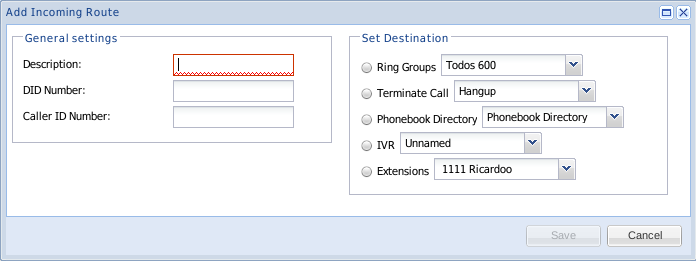
\includegraphics[scale=0.6]{screenshots/etvoip_pbx_inbound_routes_add.png}
        \caption{Inbound route creation window}
        \label{fig:etvoip_pbx_inbound_routes_add}
        \end{center}
\end{figure}

\subsubsection{Edit route}
To edit a route you must select the desired route and click on \emph{Edit route} option. Then, you will see a confirmation window (see Figure \ref{fig:etvoip_pbx_inbound_routes_add}) filled with the definitions of the route.
The parameters are identical to those provided in section \ref{sec:etvoip_pbx_inbound_routes_add}.

\subsubsection{Remover rota}
To remove a selected route entry click on \emph{Remove route} option.
A window will appear confirming the removal (Figure \ref{fig:etvoip_pbx_inbound_routes_remove}). After removal and if you do not want to perform any other operation, you must apply the changes made - \emph{Apply changes} option.

\begin{figure}[H]
        \begin{center}
        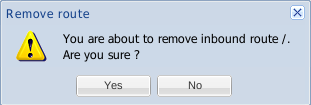
\includegraphics[scale=0.6]{screenshots/etvoip_pbx_inbound_routes_remove.png}
        \caption{Remove inbound route}
        \label{fig:etvoip_pbx_inbound_routes_remove}
        \end{center}
\end{figure}

